\documentclass[final,hyperref={pdfpagelabels=false}]{beamer}
\usepackage{grffile}
\mode<presentation>{\usetheme{I6pd2}}
\usepackage[english]{babel}
\usepackage{amsmath,amsthm, amssymb, latexsym}
\usepackage{tikz}
\usetikzlibrary{shapes.geometric, arrows,backgrounds,fit}
\usepackage{booktabs}
\usepackage{caption}
\captionsetup{justification={justified}}
\usepackage[square,numbers]{natbib}
\usepackage{ragged2e}
\tikzstyle{arrow} = [thick,line width=0.8mm,->,>=stealth]
\usepackage{hyperref}

\boldmath
\usepackage[orientation=portrait,size=a0,scale=1.4,debug]{beamerposter}


\usepackage{array,booktabs,tabularx}
\newcolumntype{Z}{>{\centering\arraybackslash}X} % centered tabularx columns
\newcommand{\pphantom}{\textcolor{ta3aluminium}} % phantom introduces a vertical space in p formatted table columns??!!
\setbeamercolor{background canvas}{bg=lightgray}
\setbeamercolor*{block body}{bg=white, fg=black}
\listfiles

\graphicspath{{figures/}}

%%%%%%%%%%%%%%%%%%%%%%%%%%%%%%%%%%%%%%%%%%%%%%%%%%%%%%%%%%%%%%%%%%%%%%%%%%%%%%%%
% Zach added packages
\usepackage{acronym}
\newacro{HI}{Hello World!}
\newacro{ASR}{Automatic Speech Recognition}
\newacro{STOI}{Short Time Objective Intelligibility Measure}
\newacro{PESQ}{Perceptual Evaluation of Speech Quality}

\usepackage{todonotes}
%%%%%%%%%%%%%%%%%%%%%%%%%%%%%%%%%%%%%%%%%%%%%%%%%%%%%%%%%%%%%%%%%%%%%%%%%%%%%%%%

\title{\huge Single Channel Dereverberation with U-Nets}
\author{Zachary Neveu (s191344)}
\institute[Department]{\small DTU Compute}
\date[July. 21-25th, 2017]{July. 21-25th, 2017}

%%%%%%%%%%%%%%%%%%%%%%%%%%%%%%%%%%%%%%%%%%%%%%%%%%%%%%%%%%%%%%%%%%%%%%%%%%%%%%%%
\newlength{\columnheight}
\setlength{\columnheight}{105cm}

\begin{document}

\begin{frame}
 \begin{columns}
% ---------------------------------------------------------%
% Set up  COLUMN 1
% ---------------------------------------------------------%
 \begin{column}{.49\paperwidth}
 \begin{beamercolorbox}[center,wd=\textwidth]{postercolumn}
 \begin{minipage}[T]{.99\textwidth}  % tweaks the width, makes a new \textwidth
 \parbox[t][\columnheight]{\textwidth}{ % must be some better way to set the the height, width and textwidth simultaneously
                                                            % Since all columns are the same length, it is all nice and tidy.  You have to get the height empirically

% ---------------------------------------------------------%
% set up block  INTRODUCTION
% ---------------------------------------------------------%
\begin{block}{Introduction}
 \begin{columns}
 \begin{column}{1\textwidth}

\centering
\begin{minipage}[t]{0.98\textwidth}

\small{In real world environments, speech is heard as a mix of direct signal with reflections caused by the surrounding environment. Late reflections decrease speech intelligibility, causing problems for listeners, as well as tasks such as \ac{ASR} \todo{cite}. Using multiple microphones, reverberation can be removed by exploiting the spatial differences between direct and reverberant sound, however this requires increased hardware cost. An algorithm is then required which can remove the effects of reverberation using only a single channel of audio. Traditional signal processing approaches can solve this problem, however these algorithms typically do not leverage the structure of speech, as this is difficult to model mathematically. Neural networks have the capability to learn the structure of speech from data, potentially allowing for superior performance to traditional algorithms.
}

\end{minipage} \hspace{1cm}


      
\end{column}
 \end{columns}
 \end{block}
 \vfill


% ---------------------------------------------------------%
% set up block  DATA
% ---------------------------------------------------------%

 \begin{block}{Key points}
 \begin{columns}
 \begin{column}{1\textwidth}
 


\vspace{-0.5cm}

\begin{minipage}[t]{0.98\textwidth}
\begin{itemize}
\small{
	\item Two neural architectures are developed for single-channel speech dereverberation: one end-to-end network, one frequency domain network.
	\item Both models are trained on the same data
	\item Losses, as well as \ac{STOI} and \ac{PESQ} measures are calculated
	\item Directions for future improvements are considered.
}
\end{itemize}


\end{minipage} 


\vspace{0.5cm}

					
          
\end{column}
\end{columns}
\vskip-1ex
\end{block}
\vfill




% ---------------------------------------------------------%
% set up block  MODEL
% ---------------------------------------------------------%

 \begin{block}{Model Architecture}
 \begin{columns}
 \begin{column}{1\textwidth}


%\vspace{0.5cm}

%\begin{minipage}[t]{0.96\textwidth}
			

\hspace{0.5cm} 

\begin{tabular}{|c|c|}
\hline
\begin{figure}
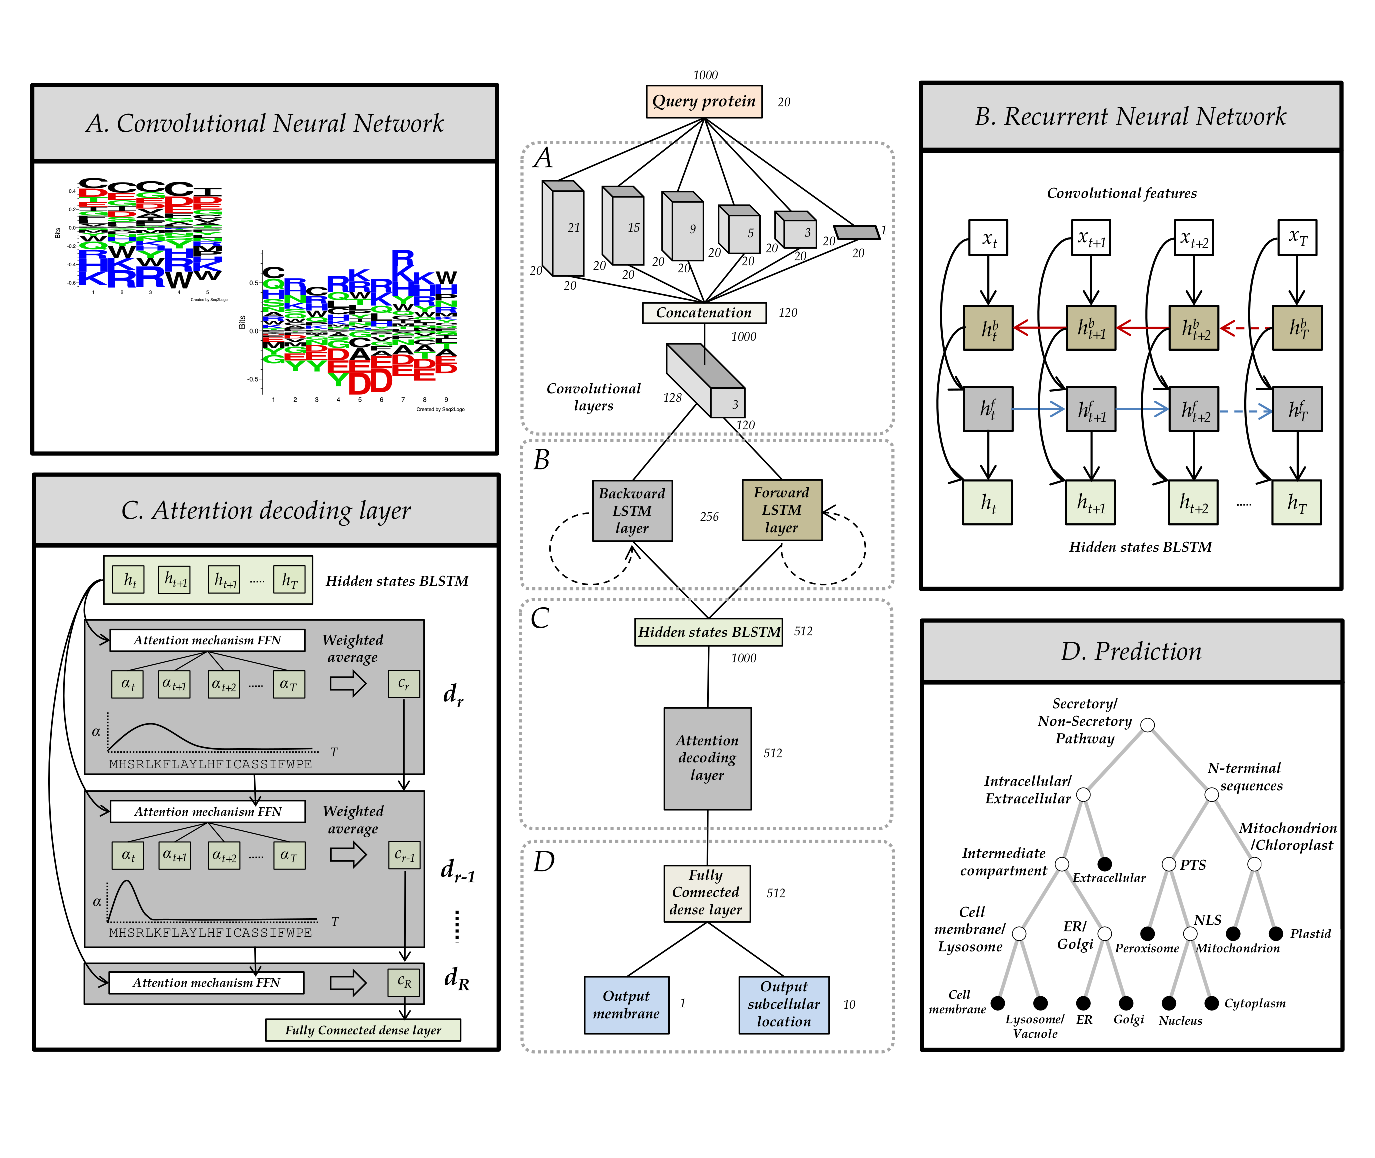
\includegraphics[width=0.5textwidth]{architecture}
 \caption{Model architecture}
\end{figure}  
& 
\begin{figure}[h]
	\centering
	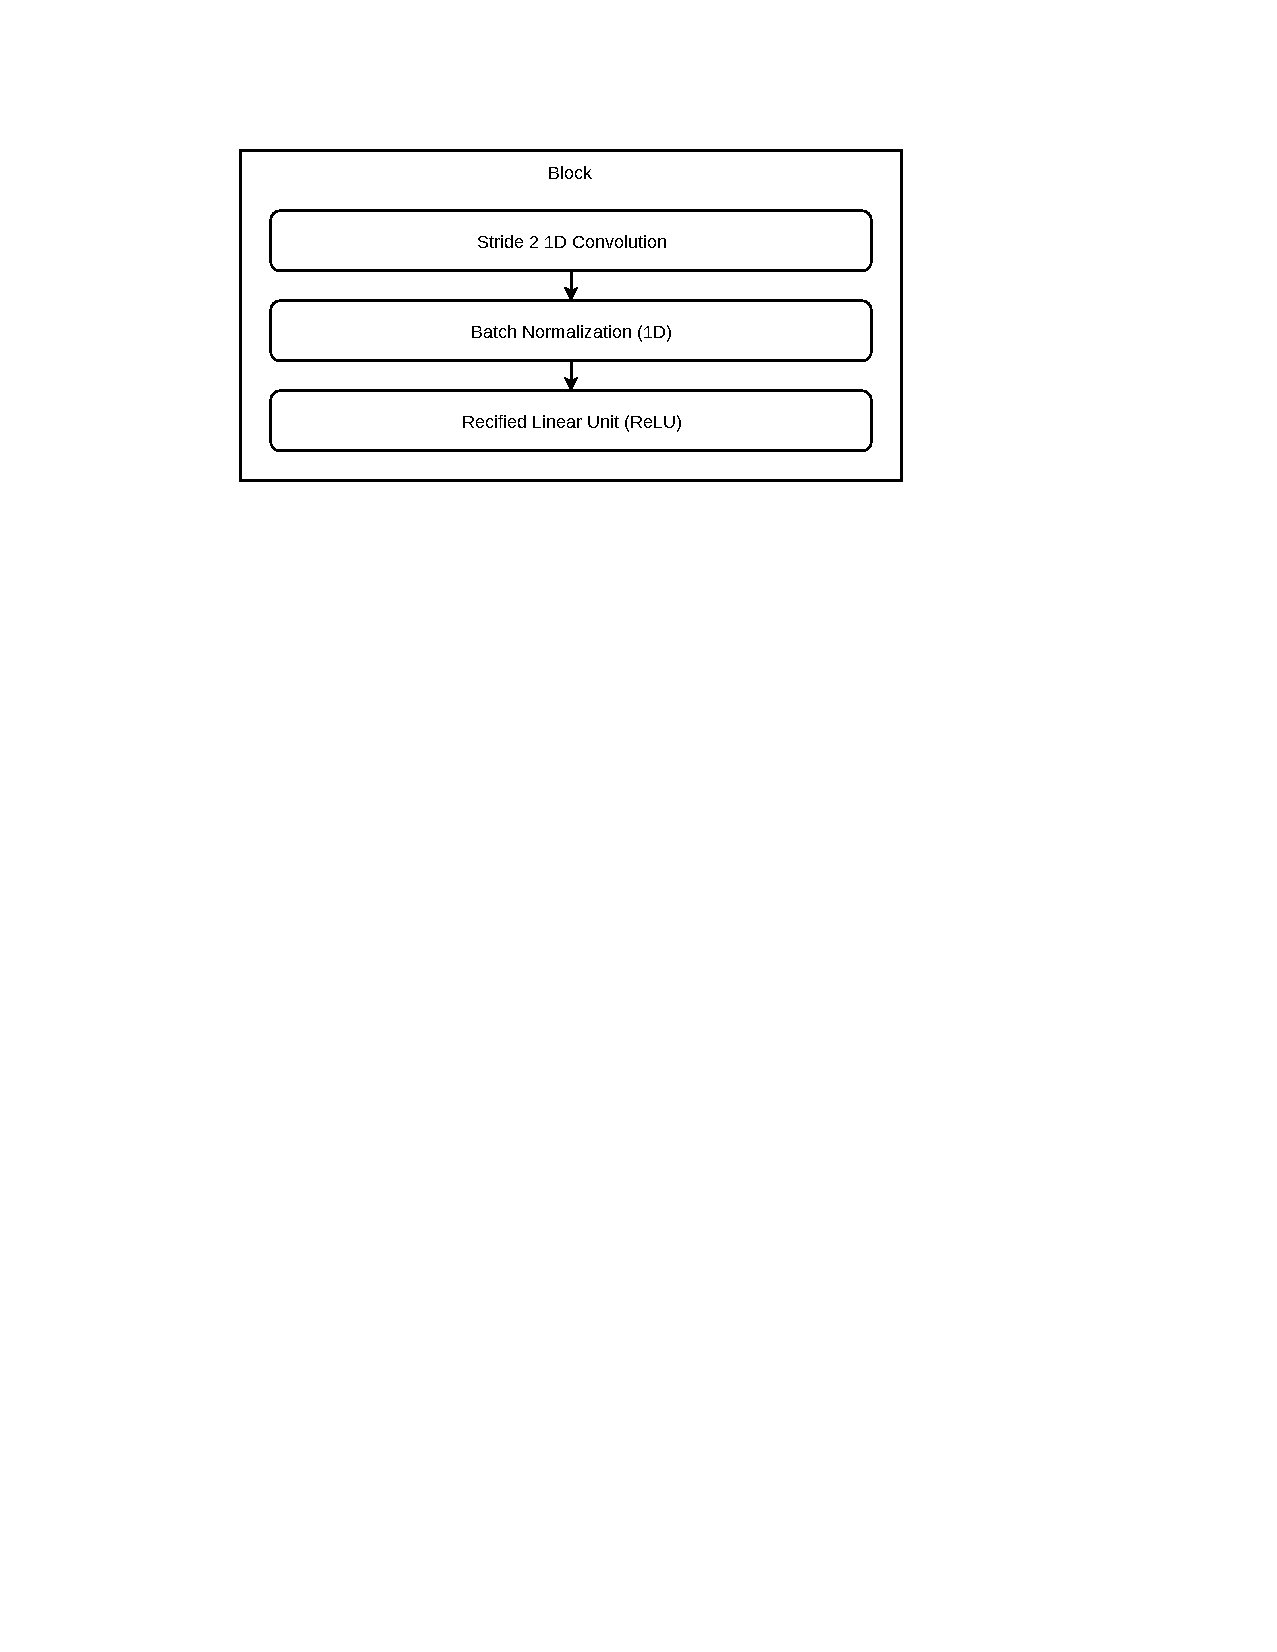
\includegraphics[width=0.8\textwidth]{block}
	\caption{Block Architecture}
	\label{fig:block}
\end{figure}
\hline
\end{tabular}

%\end{minipage}



\vspace{0.5cm}

					
                  
\end{column}
\end{columns}
\vskip-1ex
\end{block}

\vfill

 \begin{block}{Datasets comparison}
 \begin{columns}
 \begin{column}{1\textwidth}


%\vspace{0.5cm}

\centering
\begin{minipage}[t]{0.96\textwidth}
			

\hspace{0.5cm} 
 %\small{We compared the generalization performance of models trained on either the DeepLoc or the Höglund datasets. When training on the DeepLoc dataset, the model obtained an accuracy of 0.7511 on the DeepLoc test set and an accuracy of 0.8301 on the Höglund test set. An identical model trained on the Höglund dataset achieved an accuracy of 0.9138 on the Höglund test set and accuracy of 0.6426 on the DeepLoc test set. This shows that models trained on the Höglund dataset have poor generalization performance on our new dataset, which reflects the high level of homology and possibly erroneous annotations in this dataset. This is further corroborated on Figure 2, for the Höglund trained model, all locations are almost perfectly separated implying that there is little variation within the Höglund dataset classes and that the training and test sets are relatively similar. }
\vspace{-1cm}
\begin{columns}
 \begin{column}{0.45\textwidth}
 \justifying
 \small{Table 1 shows that models trained on the Höglund dataset have poor generalization performance on our new dataset, which reflects the high level of homology and possibly erroneous annotations in this dataset. This is further corroborated on Figure 2,  for the Höglund trained model, all locations are almost perfectly separated.}
 \end{column}
 \begin{column}{0.49\textwidth}

\begin{table}[h]
\small
\centering
\caption{Comparison of generalization performances between the DeepLoc dataset and the H{\"o}glund dataset.} 
\label{res:data}
\begin{tabular}{llllll}
\toprule
Training set  & Test set        & Accuracy     & Gorodkin    \\
\midrule
DeepLoc       &  DeepLoc        & 0.7511       & 0.6988    \\
H{\"o}glund	  & DeepLoc         & 0.6426       & 0.5756    \\
\hline
DeepLoc	      & H{\"o}glund     & 0.8301       & 0.8010    \\
H{\"o}glund   &  H{\"o}glund    & 0.9138       & 0.8979    \\
\bottomrule
\end{tabular}
\end{table}

 \end{column}
 \end{columns}
 
 \begin{figure}
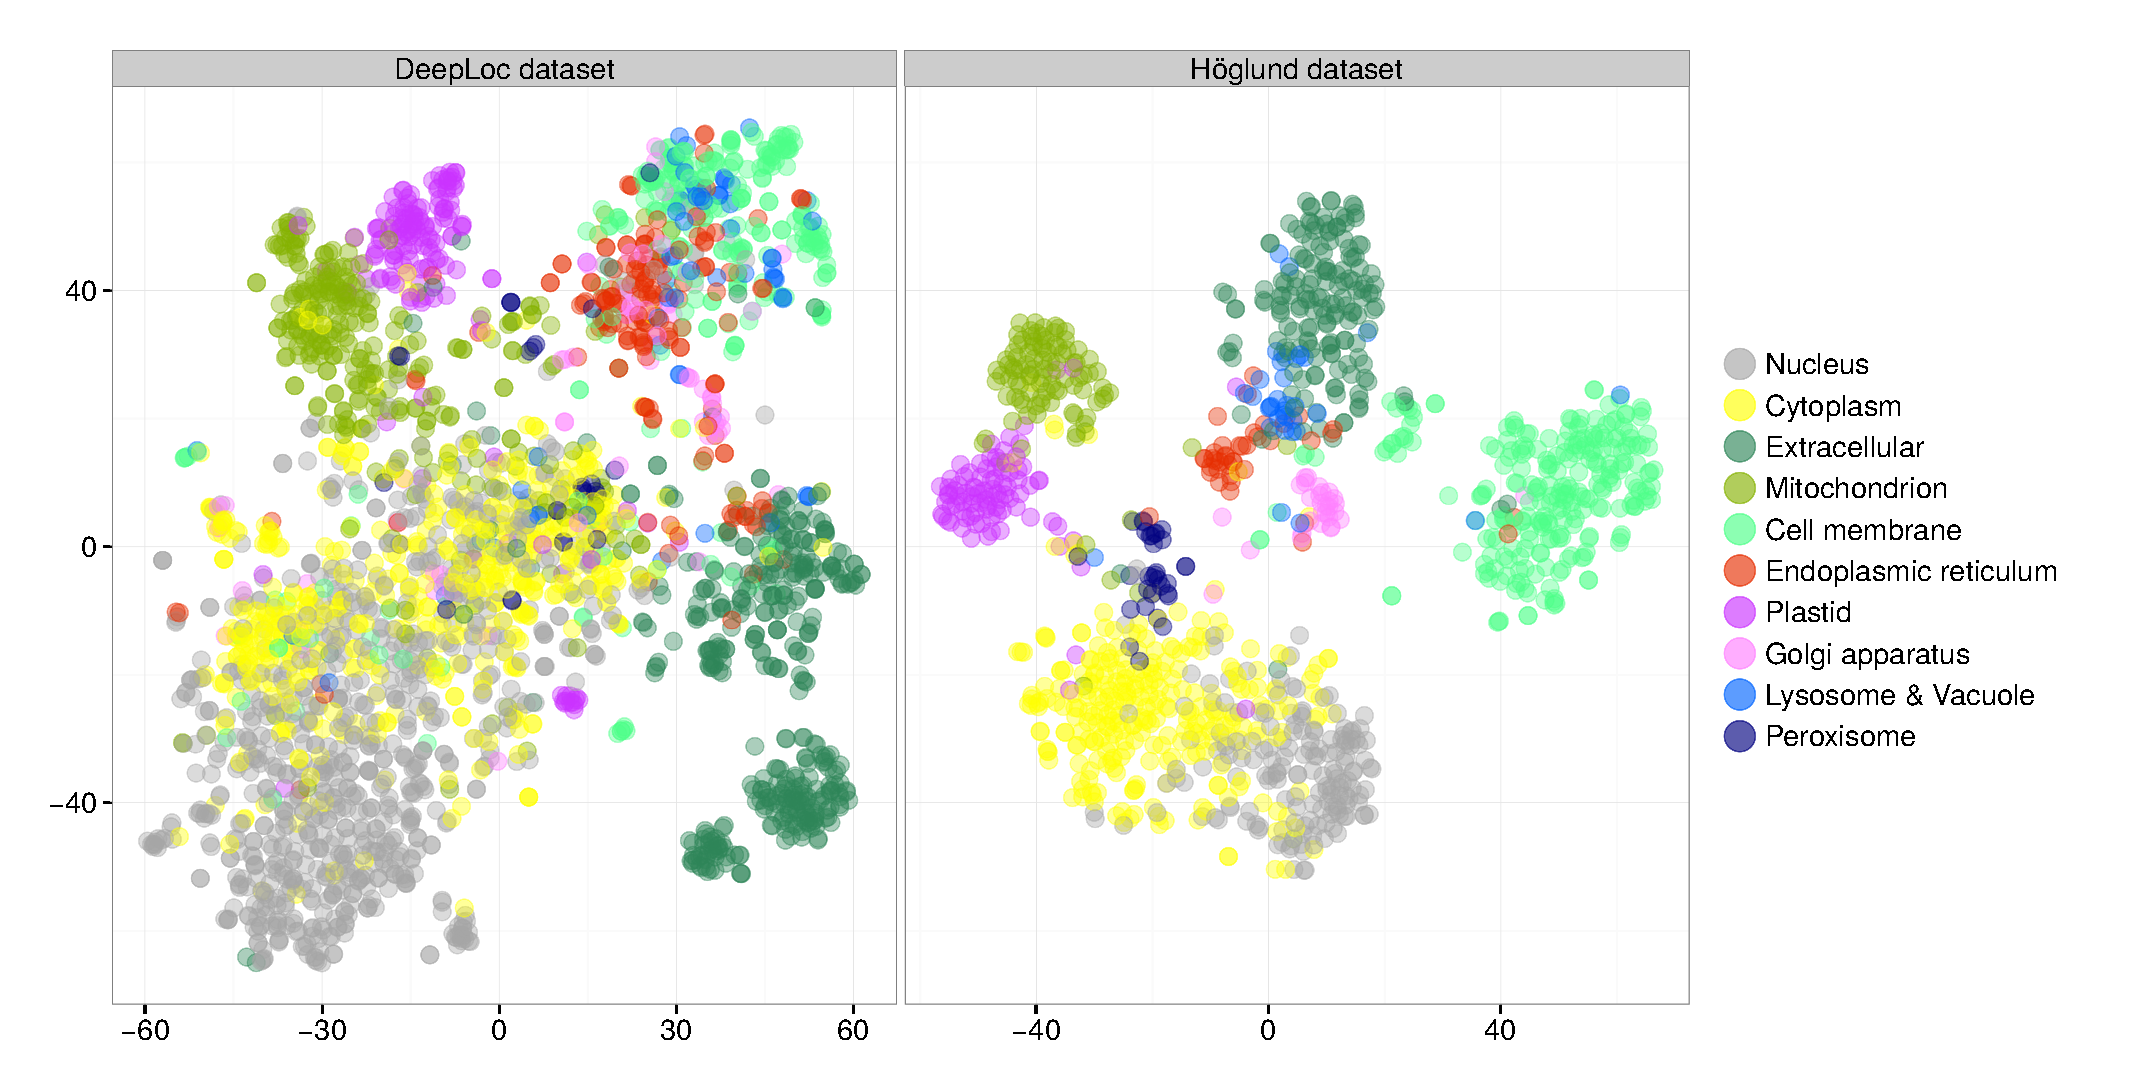
\includegraphics[width=0.95\linewidth]{tSNE_representation.eps}
 \caption{t-SNE representation of the context vector for the model trained on the DeepLoc and Höglund dataset and visualized for the respective test sets.}
\end{figure} 
\end{minipage}



\vspace{0.5cm}

					
                  
\end{column}
\end{columns}
\vskip-1ex
\end{block}
\vfill


% ---------------------------------------------------------%
% set up block REFERENCES
% ---------------------------------------------------------%



}
\end{minipage}
\end{beamercolorbox}
\end{column}
% ---------------------------------------------------------%
% end the COLUMN 1
% ---------------------------------------------------------%
 

% ---------------------------------------------------------%
% Set up COLUMN 2
% ---------------------------------------------------------%
    
\begin{column}{.49\paperwidth}
\begin{beamercolorbox}[center,wd=\textwidth]{postercolumn}
\begin{minipage}[T]{.99\textwidth} % tweaks the width, makes a new \textwidth
\parbox[t][\columnheight]{\textwidth}{ % must be some better way to set the the height, width and textwidth simultaneously
            											% Since all columns are the same length, it is all nice and tidy.  You have to get the height empirically
            
% ---------------------------------------------------------%
% set up block RESULTS + DISCUSSION
% ---------------------------------------------------------%

 \begin{block}{Model performance}
 \begin{columns}
 \begin{column}{1\textwidth}


\vspace{-1cm}

\centering
\begin{minipage}[t]{0.96\textwidth}
			
\begin{columns}
\begin{column}{0.30\textwidth} 
\justifying
\small{The accuracy of the final DeepLoc model using the new dataset is significantly better than all other methods with iLoc-Euk achieving the second best accuracy.}
\end{column}
\begin{column}{0.59\textwidth}
\begin{table}[h]
\small
\centering
\caption{Accuracy and Gorodkin measure \citep{gorodkin2004comparing} achieved by current predictors and the final DeepLoc model on the DeepLoc test set.\label{Res:current}}
\begin{tabular}{p{9cm}p{6cm}p{6cm}}
\toprule
Method & Accuracy &  Gorodkin \\
\midrule
LocTree2 & 0.6120 & 0.5250 \\
MultiLoc2 & 0.5592 & 0.4869 \\
SherLoc2 & 0.5815 & 0.5112 \\
YLoc & 0.6122 & 0.5330 \\
CELLO & 0.5521 & 0.4543 \\
iLoc-Euk & 0.6820 & 0.6412 \\
WoLF PSORT & 0.5671 & 0.4785 \\
DeepLoc & \textbf{0.7797} & \textbf{0.7347} \\
\bottomrule
\end{tabular}
\end{table}
\end{column}
\end{columns}


\end{minipage}



\vspace{0.5cm}

					
                  
\end{column}
\end{columns}
\vskip-1ex
\end{block}

\vfill

\begin{block}{Performance for each location}

\begin{columns}
\begin{column}{1\textwidth}

\centering

%\vspace{2.5cm}
\centering
\begin{minipage}[t]{.95\textwidth}


\vspace{-1cm}
\begin{table}[h]
\small
\caption{Confusion matrix of the test set on the final DeepLoc model using profiles encoding. Sens. = Sensitivity, MCC = Matthews Correlation Coefficient}
\begin{tabular}{p{8cm}p{2cm}p{2cm}p{2cm}p{2cm}p{2cm}p{2cm}p{2cm}p{2cm}p{2cm}p{2cm}p{2.5cm}p{2.5cm}}
\toprule
Location      & \multicolumn{10}{l}{Number of predicted proteins}        & Sens. & MCC \\
\midrule
Nucleus          & 680 & 103 & 4   & 5   & 2   & 8   & 1   & 2  & 2 & 1 & 0.842 & 0.784 \\
Cytoplasm         & 94  & 361 &  7  & 18  & 5   & 4   & 3   & 8  & 1 & 7 & 0.711 & 0.608 \\
Extracellular    & 3   & 5   & 365 &  5  & 5   & 4   & 2   & 0  & 4 & 0 & 0.929 & 0.907 \\
Mitochondrion     & 9   & 21  & 0   & 247 &  0  & 5   & 14  & 2  & 1 & 3 & 0.818 & 0.812 \\
Cell membrane     & 5   & 15  & 6   & 1   & 203 & 20  & 1   & 4  & 18& 0 & 0.744 & 0.732 \\
Endoplasmic ret.               & 3   & 6   & 6   & 3   & 18  & 120 &  1  & 7  & 8 & 1 & 0.694 & 0.654 \\
Plastid           & 1   & 2   & 0   & 8   & 0   & 0   & 140 &  0 & 1 & 0 & 0.921 & 0.883 \\
Golgi apparatus  & 4   & 17  & 1   & 0   & 9   & 8   & 1   & 26 & 4 & 0 & 0.371 & 0.414 \\
Lysosome/Vacuole & 0   & 7   & 11  & 1   & 20  & 9   & 0   & 4  & 12& 0 & 0.188 & 0.194 \\
Peroxisome       & 0   & 13  & 0   & 4   & 1   & 4   & 0   & 0  & 0 & 8 & 0.267 & 0.321 \\
\bottomrule

\end{tabular}
\end{table}


\end{minipage}

\end{column}
\end{columns}
\end{block}

\vfill

\begin{block}{Attention mechanism visualization}

\begin{columns}
\begin{column}{1\textwidth}

\centering

%\vspace{2.5cm}
\centering
\begin{minipage}[t]{.95\textwidth}


\vspace{-0.5cm}

\small{We are able to represent what regions in the sequence are relevant for each subcellular localization to perform the prediction.}

\vspace{0.4cm}
\begin{figure}
\centering
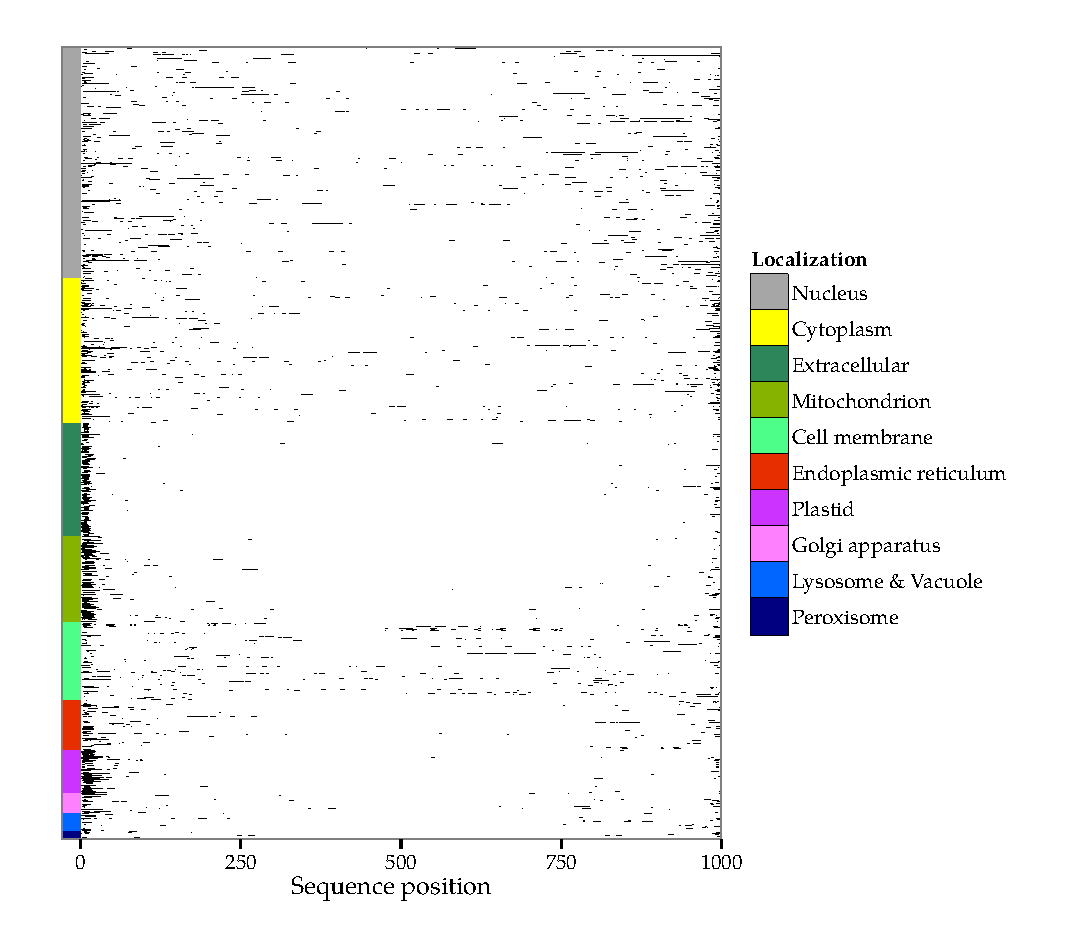
\includegraphics[width=0.9\linewidth]{Sequence_importance.eps}
 \caption{Sequence importance across the protein sequence of DeepLoc test set when making the prediction.}
\end{figure}  


\end{minipage}

\end{column}
\end{columns}
\end{block}	

\vfill

\begin{block}{Acknowledgements}
\centering
\begin{minipage}[t]{0.98\textwidth}

\small{The authors wish to thank Konstantinos Tsirigos and Arne Elofsson of Stockholm University for permission to use their fast profile construction method in DeepLoc, even though it has not been published yet. In addition, we want to thank Fabian Aicheler of University of Tübingen for kindly running the DeepLoc test set on YLoc.}
\end{minipage}
\end{block}
\vfill
\begin{block}{References}

{\footnotesize
\bibliographystyle{abbrvnat}	
\bibliography{biblio}
}			
\end{block}
\vfill


         
}
\end{minipage}
\end{beamercolorbox}
\end{column}
\end{columns}
% ---------------------------------------------------------%
% end the COLUMN 2
% ---------------------------------------------------------%
  
  
\end{frame}
\end{document}
